%%
%% This is file `sample-sigconf.tex',
%% generated with the docstrip utility.
%%
%% The original source files were:
%%
%% samples.dtx  (with options: `all,proceedings,bibtex,sigconf')
%% 
%% IMPORTANT NOTICE:
%% 
%% For the copyright see the source file.
%% 
%% Any modified versions of this file must be renamed
%% with new filenames distinct from sample-sigconf.tex.
%% 
%% For distribution of the original source see the terms
%% for copying and modification in the file samples.dtx.
%% 
%% This generated file may be distributed as long as the
%% original source files, as listed above, are part of the
%% same distribution. (The sources need not necessarily be
%% in the same archive or directory.)
%%
%%
%% Commands for TeXCount
%TC:macro \cite [option:text,text]
%TC:macro \citep [option:text,text]
%TC:macro \citet [option:text,text]
%TC:envir table 0 1
%TC:envir table* 0 1
%TC:envir tabular [ignore] word
%TC:envir displaymath 0 word
%TC:envir math 0 word
%TC:envir comment 0 0
%%
%% The first command in your LaTeX source must be the \documentclass
%% command.
%%
%% For submission and review of your manuscript please change the
%% command to \documentclass[manuscript, screen, review]{acmart}.
%%
%% When submitting camera ready or to TAPS, please change the command
%% to \documentclass[sigconf]{acmart} or whichever template is required
%% for your publication.
%%
%%
\documentclass[sigconf]{acmart}
%%
%% \BibTeX command to typeset BibTeX logo in the docs
\AtBeginDocument{%
  \providecommand\BibTeX{{%
    Bib\TeX}}}

%% Rights management information.  This information is sent to you
%% when you complete the rights form.  These commands have SAMPLE
%% values in them; it is your responsibility as an author to replace
%% the commands and values with those provided to you when you
%% complete the rights form.
\setcopyright{acmlicensed}
\copyrightyear{2018}
\acmYear{2018}
\acmDOI{XXXXXXX.XXXXXXX}
%% These commands are for a PROCEEDINGS abstract or paper.
\acmConference[ASIA CCS '26]{Make sure to enter the correct
  conference title from your rights confirmation email}{June 01--05,
  2026}{Bangalore, India}
%%
%%  Uncomment \acmBooktitle if the title of the proceedings is different
%%  from ``Proceedings of ...''!
%%
%%\acmBooktitle{Woodstock '18: ACM Symposium on Neural Gaze Detection,
%%  June 03--05, 2018, Woodstock, NY}
\acmISBN{978-1-4503-XXXX-X/2018/06}


%%
%% Submission ID.
%% Use this when submitting an article to a sponsored event. You'll
%% receive a unique submission ID from the organizers
%% of the event, and this ID should be used as the parameter to this command.
%%\acmSubmissionID{123-A56-BU3}

%%
%% For managing citations, it is recommended to use bibliography
%% files in BibTeX format.
%%
%% You can then either use BibTeX with the ACM-Reference-Format style,
%% or BibLaTeX with the acmnumeric or acmauthoryear sytles, that include
%% support for advanced citation of software artefact from the
%% biblatex-software package, also separately available on CTAN.
%%
%% Look at the sample-*-biblatex.tex files for templates showcasing
%% the biblatex styles.
%%

%%
%% The majority of ACM publications use numbered citations and
%% references.  The command \citestyle{authoryear} switches to the
%% "author year" style.
%%
%% If you are preparing content for an event
%% sponsored by ACM SIGGRAPH, you must use the "author year" style of
%% citations and references.
%% Uncommenting
%% the next command will enable that style.
%%\citestyle{acmauthoryear}


%%
%% end of the preamble, start of the body of the document source.
\begin{document}

%%
%% The "title" command has an optional parameter,
%% allowing the author to define a "short title" to be used in page headers.
\title{POSTER: GEM-PLI Side Channel in GPON: Inferring Encrypted Streaming Traffic}

%%\author{Hyunjun An}
%%\affiliation{%
%%  \institution{Heungdeok High School}
%%}
%%\email{hjahn@anhyunjun.com}

%%\renewcommand{\shortauthors}{An}

\begin{abstract}
Gigabit Passive Optical Networks (GPON), an ITU-T standardized technology adopted in FTTH networks, supports downstream payload encryption to protect subscribers' traffic. Unfortunately, encryption does not cover all access layer metadata. This poster presents a preliminary analysis demonstrating that the Payload Length Indicator (PLI), which remains in plaintext in GEM headers, can be exploited as a side channel to infer streaming activity. Using a GPON downstream simulator, We demonstrate that PLI traces are highly consistent across repeated runs of the same Youtube video and suggest that a passive attacker on the same optical splitter as the victim could potentially infer a victim's streaming activity (e.g., Youtube Video Identification).
\end{abstract}

%%HJ\ccsdesc{Do Not Use This Code~Generate the Correct Terms for Your Paper}

\begin{CCSXML}
<ccs2012>
   <concept>
       <concept_id>10003033.10003039</concept_id>
       <concept_desc>Networks~Network protocols</concept_desc>
       <concept_significance>500</concept_significance>
       </concept>
   <concept>
       <concept_id>10003033.10003039.10003044</concept_id>
       <concept_desc>Networks~Link-layer protocols</concept_desc>
       <concept_significance>500</concept_significance>
       </concept>
 </ccs2012>
\end{CCSXML}

\ccsdesc[500]{Networks~Network protocols}
\ccsdesc[500]{Networks~Link-layer protocols}

\keywords{GPON, encrypted traffic analysis, side-channel inference, video identification, passive optical networks}

%% (Removed sample teaser/received blocks; content-only change.)

\maketitle

\section{Introduction And Motivation}
As fiber internet has become dominant in network infrastructures, GPON--one of the passive optical network (PON) technologies--is adopted by many ISPs to provide fiber-to-the-home (FTTH) internet. Since GPON is a popular PON technology, it is important to ensure traffic confidentiality. 
 GPON supports AES-based downstream payload encryption at the GPON Encapsulation Method (GEM) layer. However, some fields in the GEM header remain plaintext such as the Payload Length Indicator (PLI) field used for multiplexing and the Port-ID field used for mapping subscribers' Optical Network Terminals/Units(ONTs/ONUs) (typically called "modem").

Such plaintext fields may appear innocuous. However, recent studies have demonstrated that such metadata may be exploited to infer a victim's activity (e.g., identifying a victim's web-based video streaming watching activity) ~\cite{bae-sec22}~\cite{ytyt}~\cite{ytyt2}.

A limitation in many prior optical-communication security studies is that an adversary must physically install an in-line optical tap at some point along the link to observe the victim's traffic. In contrast, GPON downstream traffic is broadcast over a passive splitter; thus, an attacker who is connected to the same splitter can receive downstream transmissions without deploying an additional in-line tap.

While prior studies primarily focused on upper layer or cellular traffic analysis~\cite{bae-sec22}~\cite{ytyt}, we researched whether the plaintext PLI field in GEM headers can be exploited to infer a victim's streaming activity.

In this poster, We developed a software-based GPON downstream simulator to analyze the statistical properties of PLI traces. Using these PLI traces, we present preliminary evidence that Youtube streaming traces are highly consistent over time and distinctive at the GEM layer, suggesting that value of the PLI field can be exploited to infer victim's video streaming.

\section{Background}  
\textbf{GPON framing.}
In GPON, the Optical Line Terminal (OLT) broadcasts downstream traffic over a passive optical splitter to multiple Optical Network Units (ONUs) (typically called "modem"). Downstream transmission is organized into fixed duration GTC frames (125~$\mu$s), each composed of a physical control block downstream (PCBd) followed by a downstream GTC payload region.
~\cite{itu-g9843} % Fig. 8-1 / 8-2

\textbf{GEM and plaintext metadata.}
Upper layer traffic (e.g., Ethernet frame) is carried in the Payload Field in GEM frames. A GEM frame starts with a 5 byte GEM header containing a 12 bit PLI, a 12 bit Port-ID, a 3 bit Payload Type Indicator (PTI), and a header error control (HEC) field. PTI indicates whether the payload is the end of a fragmented payload or not. %
~\cite{itu-g9843} % Fig. 8-11 + PLI/PTI text

\textbf{PLI length even under encryption.}
In GPON, downstream user traffic is carried as GEM frames multiplexed in the GTC payload~\cite{itu-g9843}.
Each GEM header includes a plaintext PLI field that specifies the payload length $L$ in bytes (up to 4095 bytes). In certain cases, larger payload values are fragmented accordingly~\cite{itu-g9843}(where PTI is used to indicate whether a GEM payload is a end of a fragment or not).
Downstream GEM encryption only encrypts payload field(not GEM header) using AES-CTR.
Since AES-CTR Encryption is length-preserving. even when payload bytes are encrypted, an attacker can observe the plaintext payload length.

\textbf{Video Identification.} HTTP Adaptive Streaming (HAS) is the popular video streaming model -- which is generally adopted by video streaming platforms (e.g., Youtube) --delivers video by letting the client periodically request short media segments at a bitrate chosen by an adaptive bitrate (ABR) algorithm. This request--response process forms characteristic bursty download patterns and bitrate-dependent segment sizes, which can be exploited for traffic inference.~\cite{bae-sec22}

\section{Threat Model}
We consider an attacker who is on the same optical splitter as the victim and has the capability to obtain the victim’s Port-ID, which is crucial for targeting specific GEM frames.
\begin{itemize}
  \item \textbf{1. Premise} The attacker has an optical capture device (e.g., FPGA with optical TAP, modified ONU that can receive raw GTC frames) connected to splitter and passively records downstream from OLT.
the attacker does not need to register their device with OLT; so even if they use receive-only optical tap, they can entirely record downstream records without transmitting.
  \item \textbf{2. Collect GEMs} Then, attacker extracts GTC frames from downstream traffic and parses GEM frames. 
  \item \textbf{3. Convert GEM PLI to dataset} Then, the attacker filters GEM frames for a victim's Port-ID and records PLI values with timestamps.
   \item \textbf{4. Dataset format} Each record includes \texttt{t\_start\_us}, \texttt{gem\_id}, \texttt{port\_id}, and \texttt{pli}.
  \item \textbf{5. Classification via database matching} The attacker matches the captured PLI time series to a pre-collected database of PLI traces (built from known videos) and selects the closest match to infer the victim’s video.
\end{itemize}

\section{Trace Generation}
To demonstrate the threat model in our experimental environment, we developed a software based GPON downstream trace generator~\cite{github} that follows key ITU-T G.984.3 TC-layer parameters relevant to PLI (125~$\mu$s framing and GEM header formatting). From a downlink ethernet packet capture file of encrypted video traffic, we (i) map Ethernet frames into GEM payloads (fragmenting to satisfy the 12 bit PLI limit), (ii) generate plaintext GEM headers (PLI/Port-ID/PTI), and (iii) pack the GEM stream into fixed-length 125~$\mu$s downstream frames consistent with the configured line rate. The attacker signal is either the GEM-level PLI sequence or the per-frame occupancy series. Large Ethernet packets may generate multiple GEM fragments; thus, PLI values in our traces reflect per fragment payload lengths (the attacker-visible observable).

\textbf{Note.} Payload bytes can optionally be AES-CTR protected; however, this does not change the PLI trace because AES-CTR is length-preserving (XOR), so encryption does not change any fragment length. Our analysis uses only plaintext headers (e.g., PLI) and timing.

\section{Experiment and Preliminary Results}
First, we played each of 10 videos (three runs each; run1, run2, run3) on Ubuntu 24.04 under a fixed playback quality and resolution setting (720p). To minimize interference, we restricted other background traffic (e.g., VNC, SSH) during playback. For each run, we captured downlink ethernet packet (PCAP) for 180 seconds. Then, we replayed each PCAP file in our simulator to produce a CSV dataset of PLI values and timestamps(one trace per run) (e.g., vid001\_run001.gem.csv~\cite{github}). We preserve original PCAP packet timestamps to retain idle periods and burstiness; each synthesized GEM is assigned t\_start\_us derived from the PCAP time base (µs resolution). After producing the dataset, we visualized cumulative PLI--Time Plot based on our dataset(Publicly Available on our Github repository)~\cite{github}. We observed a clear correlation between each video and its cumulative PLI over time graph~\cite{github}; traces from the same video show highly consistent slopes across runs.(Our Github repository: \//out\_cumsum)

For similarity analysis, we bin PLI events into 100ms bins, compute the cumulative sum, normalize by the final cumulative value, and compare traces using Pearson correlation and RMSE.
These traces approximate the payload length observations available to a real same-splitter adversary and enable systematic evaluation of PLI based inference.
We use run1,2 dataset files as a database and run3 dataset files as a query trace.

\begin{figure}[t]
  \centering
  \begin{minipage}[t]{0.495\linewidth}
    \centering
    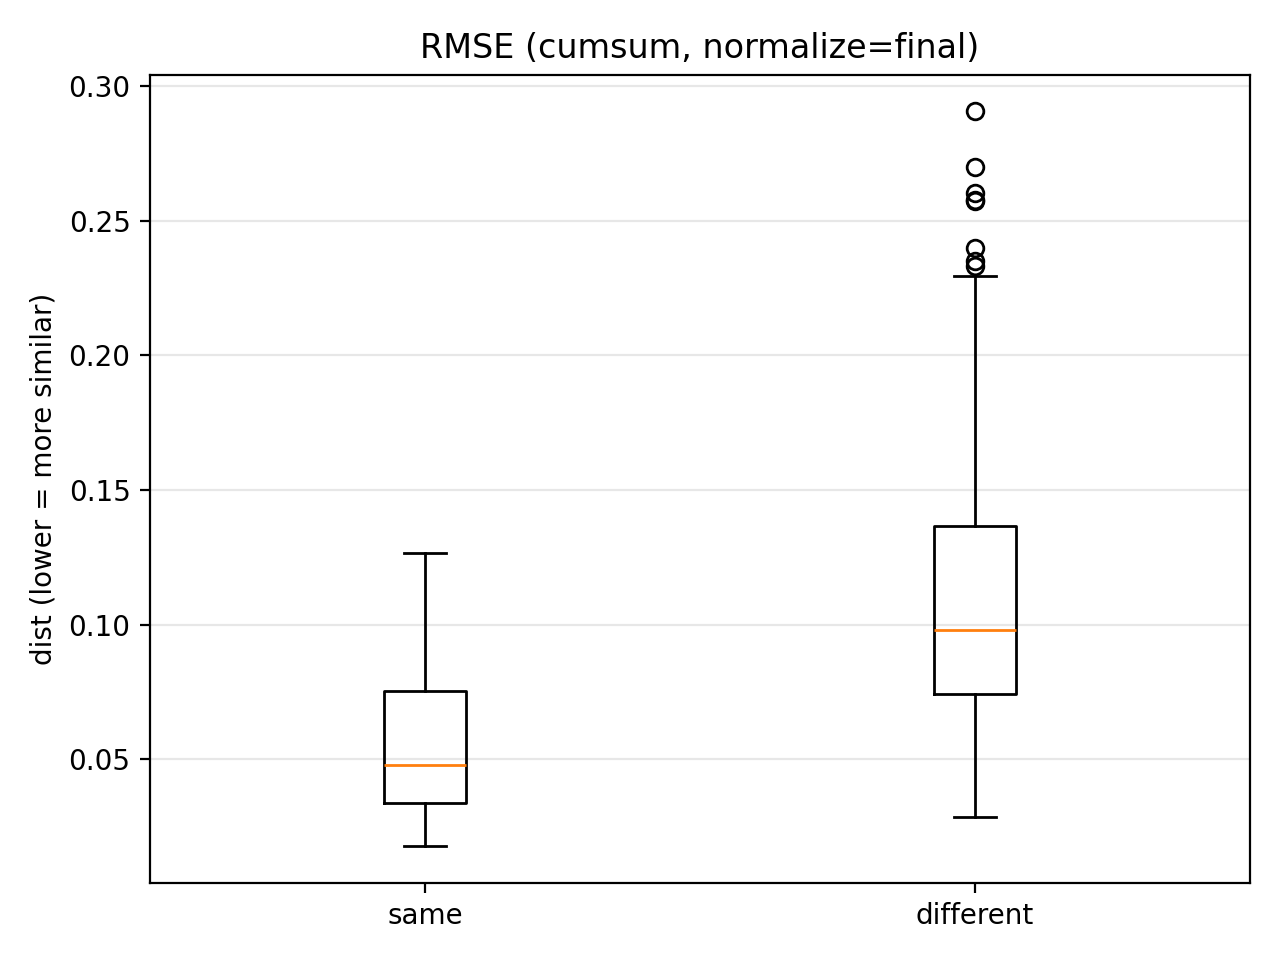
\includegraphics[width=\linewidth]{fig/box_rmse.png}\\
    \vspace{-0.3em}
    {\small (a) RMSE (lower = more similar)}
  \end{minipage}\hfill
  \begin{minipage}[t]{0.495\linewidth}
    \centering
    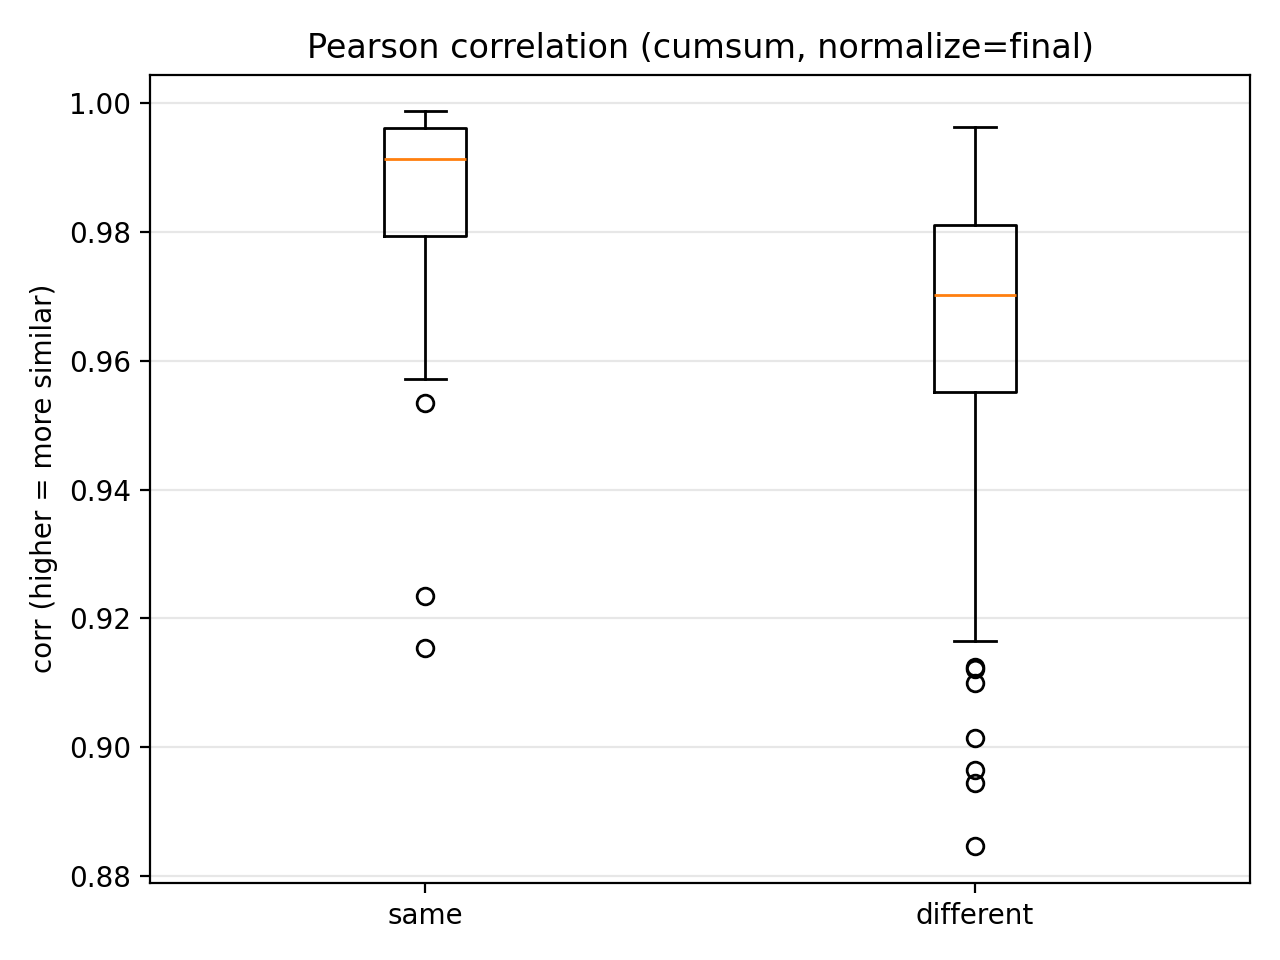
\includegraphics[width=\linewidth]{fig/box_pearson_r.png}\\
    \vspace{-0.3em}
    {\small (b) Pearson correlation (higher = more similar)}
  \end{minipage}
\caption{Similarity distributions between same-video and different-video cumulative PLI traces. Same video pairs tend to show higher correlation and RMSE smaller distance. We found a partial intersection due to ABR variability and buffering, but the distinction is sufficient for discrimination using both RMSE and Pearson}
\Description{Two box plots: (a) RMSE (lower is more similar) and (b) Pearson correlation (higher is more similar), comparing same-video versus different-video cumulative PLI traces.}

  \label{fig:pli-metrics}
\end{figure}

\begin{table}[t]
  \centering
  \small
  \setlength{\tabcolsep}{3pt}
  \renewcommand{\arraystretch}{1.0}
  \caption{Per-query Top-1 predictions.~\cite{github}}
  \label{tab:top1-detail}
  \begin{tabular}{l l c c c}
    \hline
    \textbf{Query} & \textbf{Prediction} & \textbf{CORRECT} & \textbf{margin} & \textbf{$r$/RMSE} \\
    \hline
    vid001/r3 & vid001/r1 & T & 2 & 0.998/0.025 \\
    vid002/r3 & vid002/r1 & T & 5 & 0.995/0.041 \\
    vid003/r3 & vid003/r2 & T & 1 & 0.980/0.050 \\
    vid004/r3 & vid004/r1 & T & 2 & 0.996/0.037 \\
    vid005/r3 & vid005/r2 & T & 2 & 0.998/0.020 \\
    vid006/r3 & vid008/r1 & F & 2 & 0.994/0.048 \\
    vid007/r3 & vid007/r1 & T & 2 & 0.999/0.025 \\
    vid008/r3 & vid008/r1 & T & 2 & 0.999/0.018 \\
    vid009/r3 & vid009/r2 & T & 2 & 0.990/0.041 \\
    vid010/r3 & vid010/r1 & T & 3 & 0.998/0.020 \\
    \hline
  \end{tabular}
\end{table}

We quantify similarity on the normalized cumulative PLI time series: same video pairs exhibit higher Pearson correlation (median $r=0.991$ vs $0.970$, AUC=0.779) and lower RMSE (median 0.048 vs 0.098, AUC=0.826).
Using nearest matching with rank voting over Pearson and RMSE, we achieve 90\% Top-1 identification accuracy (9/10) when matching run3 queries against run1,run2 query traces.

\section{Conclusion And Discussion}
Despite GEM Payload Encryption, GPON may remain vulnerable to streaming inference because PLI values in GEM headers can be exploited to infer a victim’s video activity (e.g., Youtube). 
Potential mitigations include traffic shaping and obfuscating GEM metadata.

Future Work will be conducted in testbed with Real OLT, ONU and Optical Splitter. We will use FPGA device to capture GEM frames to parse downstream frames. We will expand to more videos and longer captures with changing various resolution, bitrate.

\textbf{Extent to XGS-PON Networks.} We assume that XGS-PON has same issue; XGEM Frame that XGS-PON uses has Payload Length Indicator Field like GEM. We will validate this by repeating our capture-and-matching evaluation on an XGS-PON testbed.

\begin{thebibliography}{6}

\bibitem{itu-g9843}
ITU-T. Gigabit-capable passive optical networks (GPON): Transmission convergence layer specification. Recommendation G.984.3. International Telecommunication Union.

\bibitem{cisco-gpon}
Cisco. 2023. Understand GPON Technology. Cisco Troubleshooting TechNotes. Document ID: 216230. Updated December 6, 2023. \url{https://www.cisco.com/c/en/us/support/docs/switches/catalyst-pon-series/216230-understand-gpon-technology.html}. Accessed 2026-02-04.

\bibitem{github}
Gitshare link of Our Github repository. \url{https://gitshare.me/repo/c8afd178-a072-4cee-a01c-8b3d12467a28}. Accessed 2026-02-04.

\bibitem{bae-sec22}
Sangwook Bae, Mincheol Son, Dongkwan Kim, CheolJun Park, Jiho Lee, Sooel Son, and Yongdae Kim. 2022. Watching the Watchers: Practical Video Identification Attack in LTE Networks. In \emph{31st USENIX Security Symposium (USENIX Security '22)}. USENIX Association, 1307--1324. \url{https://www.usenix.org/conference/usenixsecurity22/presentation/bae}.

\bibitem{ytyt}
Xiyuan Zhang, Gang Xiong, Zhen Li, Chen Yang, Xinjie Lin, Gaopeng Gou, and Binxing Fang. 2024. Traffic spills the beans: A robust video identification attack against YouTube. \emph{Computers \& Security} 137 (2024), Article 103623. \url{https://doi.org/10.1016/j.cose.2023.103623}.

\bibitem{ytyt2}
Nan Hu, Hua Wu, Hangyu Zhao, Shanshan Ni, and Guang Cheng. 2024. Breaking Through the Diversity: Encrypted Video Identification Attack Based on QUIC Features. In \emph{Computer Security -- ESORICS 2024} (Lecture Notes in Computer Science). 166--186. \url{https://doi.org/10.1007/978-3-031-70903-6_9}.

\end{thebibliography}

\end{document}
\endinput
%%
%% End of file `sample-sigconf.tex'.